% =====================================================================
% Companion paper: Systemic Criticality in the Multiplex Alliance Economy
% =====================================================================
\documentclass[11pt,letterpaper]{article}

\usepackage[margin=0.95in]{geometry}
\usepackage{setspace}
\setstretch{1.12}

\usepackage[T1]{fontenc}
\usepackage[utf8]{inputenc}
\usepackage{microtype}

\usepackage{amsmath}
\usepackage{amssymb}
\usepackage{bm}

\usepackage{graphicx}
\graphicspath{{../../outputs/strategic/aggregate/}}
\usepackage{float}
\usepackage{caption}
\captionsetup{font=small,labelfont=bf}

\usepackage{booktabs}
\usepackage{array}

\usepackage{natbib}
\usepackage[colorlinks,citecolor=blue,linkcolor=blue,urlcolor=blue]{hyperref}

\usepackage{titlesec}
\titleformat{\section}{\normalfont\large\bfseries}{\thesection}{0.7em}{}
\titlespacing*{\section}{0pt}{1.2em}{0.4em}
\titleformat{\subsection}{\normalfont\normalsize\bfseries}{\thesubsection}{0.6em}{}
\titlespacing*{\subsection}{0pt}{0.8em}{0.25em}

\begin{document}

\begin{center}
{\LARGE\bfseries The Hidden Architecture of Corporate Interdependence:\\[0.2em]
Systemic-Criticality Mapping of the Multiplex Alliance Economy\par}
\end{center}
\vspace{1em}

\begin{abstract}
\noindent
Corporate network studies typically rank firms by their own position in
the network---degree, betweenness, eigenvector centrality.  These
measures describe what a firm \emph{has}, not what other firms are
structurally \emph{exposed to losing} if the firm vanished.  We
construct a \emph{systemic-criticality meta-network} from the
full-graph strategic alliance panel, using canonical ultimate-parent
CUSIP-6 identifiers and partner-specific vulnerability scores.  The corrected 2017 snapshot
contains 7{,}626 generated focal-firm reports, 1{,}754 active focal
firms with non-empty dependency portfolios, 4{,}918 focal-partner
candidate dependencies, and 3{,}690 top-5 directed critical-dependency
edges across 2{,}939 distinct critical partners.  Unlike the earlier
prototype, the new ranking is not driven by a single layer constant:
each edge combines layer-specific partner-exit weights, dyad tenure,
tie strength, redundancy, partner centrality, and a first-order
counterfactual betweenness-exposure proxy.  The top 20 systemic firms
include industrials and energy firms (General Electric, Exxon Mobil,
Royal Dutch Shell), platform and telecom firms (Alphabet, Amazon,
AT\&T), financial/holding companies (Blackstone, Berkshire Hathaway,
Carlyle), and several non-Compustat state or foreign entities.  The
analysis also reports top-$k$ sensitivity, null-model concentration,
estimator robustness, ablations, a backtest on observed exits, and a
system-removal stress test.  A downstream recommender audit further
shows that partner-level systemicity does not personalize focal-firm
partner choice: multiplicative candidate-side scores collapse to
universal candidates, and inside saturated brokerage frontiers the
candidate-side annotations even anti-correlate with realized new
$L_2$ partner selections.  The central conclusion is more cautious
than the prototype: the meta-network is a structural dependency map
and stress-testing device, not direct evidence that every top-ranked
partner exit would causally destroy value, and not a standalone
firm-level recommender.
\end{abstract}

% =====================================================================
\section{Introduction}

No firm is an island.  When a corporation forms an alliance with a
partner, it absorbs a piece of the partner's exposure: the partner's
innovations flow through it, the partner's distribution channels become
accessible to it, and the partner's operational routines become coupled
with its own.  Over a decade of sustained partnerships, these
absorptions compound.  The day a critical partner exits---via
acquisition, bankruptcy, strategic withdrawal, or disappearance from
the alliance economy---is the day that accumulated dependency can
collapse.

Prior empirical work on alliance networks \citep{burt1992, ahuja2000,
phelps2010} measures firms by their \emph{own} network position: who
they are connected to, how centrally they sit.  These measures are
descriptive of the firm, not of the firms that depend on it.  The
strategic pipeline developed in the companion work provides the
ingredients for a different question: \emph{Whose exit is many other
firms simultaneously structurally exposed to?}

The first prototype answered this question by aggregating top-5 rows
from per-firm vulnerability CSVs.  That prototype was useful but
overstated its empirical precision.  Two corrections are essential.
First, CUSIP fields must be canonical strings.  CSV inference split the
same partner into duplicated identities when leading zeros or numeric
CUSIPs were handled inconsistently.  Second, a layer-only loss rule
made many vulnerabilities mechanical: L$_2$ ties inherited the same
coefficient, and non-L$_2$ ties inherited a fixed fraction of it.  The
corrected pipeline rebuilds the dependency panel directly from the
typed edge and firm-year artifacts, normalizes every CUSIP-6 field, and
scores every focal-partner-year edge using partner-specific features.

Three corrected findings emerge:
\begin{enumerate}
  \item The 2017 systemic ranking is identity-clean: 2{,}939 distinct
  critical partners and zero duplicated normalized partner rows.
  \item The ranking is partner-specific rather than layer-constant.
  Top-ranked partners are those combining harmful layer exposure with
  strong dyadic tie strength, long tenure, low redundancy, high partner
  centrality, and large focal betweenness exposure.
  \item The causal interpretation is now conservative.  Legacy TWFE
  estimates recover a negative L$_2$ partner-exit coefficient
  ($-0.065$, $p=0.036$), but stacked-cohort estimates are weaker and
  even positive for L$_1$ and L$_2$.  We therefore report both and use
  the stacked-cohort estimate as the conservative reference in the main
  systemic ranking.
\end{enumerate}

% =====================================================================
\section{Method: The Systemic-Criticality Meta-Network}
\label{sec:method}

Let $\mathcal{F}_{t}$ be the set of Compustat-matched focal firms with
at least one active alliance partner in the five-year rolling window
$[t-4,t]$.  Let $P_t(f)$ be the set of all partners of focal firm $f$
in that window, where partners may be public, private, foreign-listed,
universities, state entities, or other non-Compustat organizations.
The corrected pipeline constructs one directed candidate dependency
edge for each $(f,p,t)$ with $p \in P_t(f)$, for every year
$t=1995,\ldots,2017$.

Each edge carries a predicted loss score:
\begin{equation}
  \widehat{\ell}_{fpt}
  = - \left[
      \sum_{\lambda \in \{L_1,L_2,L_3,L_4\}}
      m_{fp\lambda t} \cdot
      \max(0,-\widehat{\beta}_{\lambda})
    \right]
    \cdot
    S_{fpt},
\end{equation}
where $m_{fp\lambda t}$ is the dyad's layer mix and
$\widehat{\beta}_{\lambda}$ is the layer-specific partner-exit event
study coefficient.  The multiplier $S_{fpt}$ is the product of five
partner-specific factors,
\begin{equation}
  S_{fpt} = s^{\text{strength}}_{fpt} \cdot
            s^{\text{tenure}}_{fpt}   \cdot
            s^{\text{redundancy}}_{fpt} \cdot
            s^{\text{centrality}}_{pt} \cdot
            s^{\text{exposure}}_{fpt},
\end{equation}
each in a bounded non-negative range.  $s^{\text{strength}}_{fpt}$
is a normalized count of active dyad-deals in the rolling window;
$s^{\text{tenure}}_{fpt}$ is a sigmoid in dyad first-year age;
$s^{\text{redundancy}}_{fpt}$ discounts a partner whose layer-SIC
slot is already covered by other partners in the focal's
portfolio; $s^{\text{centrality}}_{pt}$ is the partner's
layer-betweenness percentile in year $t$; and
$s^{\text{exposure}}_{fpt}$ is the first-order counterfactual
exposure $|\Delta c^{(\lambda)}_{fpt}|$ defined below.  Exact
definitions and numerical ranges are recorded in
\texttt{strategic\_pipeline/aggregate/build\_systemic\_criticality.py}.

The first-order counterfactual exposure is:
\begin{equation}
  \Delta c^{(\lambda)}_{fpt}
  =
  - c^{(\lambda)}_{ft}
  \cdot
  \frac{w^{(\lambda)}_{fpt}}
       {\sum_{q \in P_t(f)} w^{(\lambda)}_{fqt}},
\end{equation}
with zero exposure when the focal firm has no layer-$\lambda$ strength.
This is not an exact recomputation of all-pairs betweenness after every
possible partner deletion; it is a scalable first-order exposure proxy
for the share of the focal firm's layer-specific brokerage that runs
through partner $p$.

The directed meta-network for year $t$ keeps the top five partners of
each active focal firm by $|\widehat{\ell}_{fpt}|$:
\begin{equation}
\mathcal{E}_t = \{(f,p,t): p \in \textrm{top-5 of } f
                  \textrm{ by } |\widehat{\ell}_{fpt}|\}.
\end{equation}
For each partner $p$, systemic criticality is:
\begin{align}
\textrm{in-degree}_{pt} &= |\{f : (f,p,t)\in\mathcal{E}_t\}|,\\
\textrm{total cost}_{pt} &= \sum_{f:(f,p,t)\in\mathcal{E}_t}
|\widehat{\ell}_{fpt}|.
\end{align}

\subsection{Layer-specific exit weights}

Table~\ref{tab:weights} reports the corrected layer-specific event
study estimates.  The stacked-cohort estimate is the primary
coefficient used in the main ranking; legacy TWFE is retained as an
estimator-robustness comparison.  Positive stacked-cohort coefficients
are treated as zero loss in the vulnerability score, because the
systemic map ranks downside exposure rather than gains from partner
exit.

\begin{table}[H]
\centering
\footnotesize
\caption{Layer-specific partner-exit weights.  Dependent variable is
log market value.  Event year is the first absent year after a partner
is active and then exits the alliance network.}
\label{tab:weights}
\begin{tabular}{lrrrrrr}
\toprule
Layer & TWFE $t{+}1$ & TWFE $p$ & TWFE treated
      & Stacked $t{+}1$ & Stacked $p$ & Stacked treated \\
\midrule
L1 & $-0.039$ & 0.236 & 1{,}607 & $+0.031$ & 0.368 & 1{,}607 \\
L2 & $-0.065$ & 0.036 & 1{,}913 & $+0.031$ & 0.326 & 1{,}913 \\
L3 & $-0.030$ & 0.560 &   616 & $-0.028$ & 0.629 &   616 \\
L4 & $-0.051$ & 0.135 & 1{,}770 & $-0.035$ & 0.362 & 1{,}770 \\
\bottomrule
\end{tabular}
\end{table}

% =====================================================================
\section{Findings}
\label{sec:findings}

\subsection{Identity and coverage audit}

The corrected 2017 snapshot distinguishes report generation from
active dependency coverage.  The strategic pipeline generated 7{,}626
focal-firm report directories and 7{,}626 partner-vulnerability CSVs,
but only 1{,}754 of those CSVs are non-empty in the 2017 active
five-year window.  This exactly matches the rebuilt active focal count:
1{,}754 Compustat focal firms, 4{,}918 candidate directed
focal-partner dependencies, and 3{,}690 top-5 dependency edges.

The identity fix matters.  The prototype aggregate contained 63
duplicated partner identities after CSV type inference.  The corrected
aggregate has 2{,}939 distinct 2017 critical partners and zero
duplicated normalized partner rows.

\paragraph{Per-firm reports realigned with the corrected panel.}
The original per-firm \texttt{stress.md} reports were produced before
the corrected aggregate panel existed and inherited the prototype's
layer-uniform exit cost.  All 7{,}626 reports were regenerated against
\texttt{critical\_edges\_panel.parquet} so that the per-firm and
aggregate artifacts now agree by construction.\footnote{The
  regeneration ran as two Slurm arrays of 4{,}000 and 3{,}626 tasks
  with a fifty-task concurrency throttle.  Both arrays completed with
  zero failures.}  The change is not cosmetic.  Qualcomm
(CUSIP~747525), one of the persistent top-20 partners in
Section~\ref{sec:findings}, illustrates the difference at the
per-firm level.  Under the prototype scorer, Qualcomm's top critical
partners were dominated by L$_2$ telecommunications ties (Alcatel
Lucent, ZTE, Dilithium, Egyptian Telephone) because every L$_2$
exit was assigned a uniform $-10.6\%$ market-value cost.  Under the
corrected partner-specific scorer combining stacked-cohort layer
weights with dyad tenure, tie strength, redundancy, partner centrality,
and counterfactual betweenness exposure, Qualcomm's top five become
Novartis~AG (L$_4$, $-0.0506$), WebMD Health (L$_3$, $-0.0445$),
GlaxoSmithKline (L$_3$, $-0.0434$), Alcatel Lucent (L$_4$, $-0.0384$),
and Samsung Electronics (L$_4$, $-0.0377$).  Pharma and operations
ties replace the layer-mechanical telecom answer; Alcatel Lucent
remains in the list but enters via L$_4$ with a value-weighted score
rather than via L$_2$ with a flat coefficient.

\subsection{The systemically important}

Figure~\ref{fig:m1} ranks the top 30 critical partners by total
predicted log-market-value cost.  Table~\ref{tab:top20} lists the top
20.

\begin{figure}[H]
\centering
\includegraphics[width=0.78\textwidth]{fig_m1_top_firms.png}
\caption{Top 30 systemic-critical partners and entities in the
corrected 2017 meta-network.  Bar length is aggregate predicted
log-market-value exposure across focal firms that rank the partner
in their top five.  Includes Compustat firms, sovereign/state entities,
private-equity vehicles, and foreign listings.}
\label{fig:m1}
\end{figure}

\begin{table}[H]
\centering
\footnotesize
\caption{Top 20 systemic-critical partners in the corrected 2017
meta-network.  Total cost is aggregate predicted $|\log(\mathrm{MV})|$
loss; in-degree is the number of focal firms ranking the partner in
their top five.}
\label{tab:top20}
\begin{tabular}{rlccrr}
\toprule
Rank & Partner & SIC2 & C & In-deg & Total cost \\
\midrule
1  & General Electric Co              & 36 & Y & 25 & 1.256 \\
2  & Exxon Mobil Corp                 & 29 & Y &  8 & 0.599 \\
3  & Singapore                        & 99 & N &  7 & 0.437 \\
4  & AT\&T Inc                        & 48 & Y &  7 & 0.432 \\
5  & Royal Dutch Shell PLC            & 29 & Y &  7 & 0.418 \\
6  & Alphabet Inc                     & 73 & N & 10 & 0.409 \\
7  & The Dow Chemical Co              & 28 & N &  6 & 0.388 \\
8  & Amazon.Com Inc                   & 59 & Y &  9 & 0.376 \\
9  & Kinder Morgan Energy Partners    & 49 & Y &  5 & 0.339 \\
10 & Blackstone Group LP              & 67 & N &  8 & 0.326 \\
11 & Boeing Co                        & 37 & Y &  5 & 0.311 \\
12 & Berkshire Hathaway Inc           & 63 & Y &  5 & 0.294 \\
13 & United Arab Emirates             & 99 & N &  4 & 0.288 \\
14 & Qualcomm Inc                     & 36 & Y &  7 & 0.277 \\
15 & Mitsui \& Co Ltd                 & 50 & Y &  3 & 0.273 \\
16 & Mexichem SAB de CV               & 28 & N &  3 & 0.262 \\
17 & Fluor Corp                       & 87 & Y &  5 & 0.260 \\
18 & Saudi Arabia                     & 99 & N &  3 & 0.247 \\
19 & The Carlyle Group LP             & 67 & N &  7 & 0.244 \\
20 & Total SA                         & 13 & N &  5 & 0.244 \\
\bottomrule
\end{tabular}
\end{table}

The corrected list differs materially from the prototype.  Microsoft
is no longer mechanically first because L$_2$ exposure is no longer
assigned a uniform 10.6\% cost.  Industrial and energy partners rise
because the conservative stacked-cohort weights identify downside
exposure primarily in L$_3$ and L$_4$ windows, and because these firms
combine high partner centrality with strong, persistent, low-redundancy
ties.

\subsection{Systemic role does not reduce to firm size}

Figure~\ref{fig:m2} plots each critical partner's in-degree against
its own market value.  The figure is now a diagnostic rather than a
claim of causal damage: upper-left partners are structurally
important relative to their observed scale, while upper-right partners
are both large and dependency-dense.

\begin{figure}[H]
\centering
\includegraphics[width=0.78\textwidth]{fig_m2_indegree_vs_mv.png}
\caption{In-degree versus own latest market value among critical
partners with Compustat market-value data.  Orange markers are the
top-10 systemic partners with available market value.}
\label{fig:m2}
\end{figure}

\subsection{Industry concentration of systemic criticality}

Aggregating in-degree at the two-digit SIC level
(Figure~\ref{fig:m3}) shows concentration in software/business
services (SIC~73), chemicals/pharmaceuticals (SIC~28), holding and
investment companies (SIC~67), engineering/R\&D services (SIC~87),
and electronics (SIC~36).  The SIC~99 category also appears in the
firm ranking through state/geographic entities such as Singapore,
United Arab Emirates, and Saudi Arabia; these are treated as
non-Compustat alliance participants rather than public operating
companies.

\begin{figure}[H]
\centering
\includegraphics[width=0.78\textwidth]{fig_m3_sic_heatmap.png}
\caption{Top-20 SIC-2 industries by aggregate systemic-criticality
metrics.  Color intensity is normalized within each column.}
\label{fig:m3}
\end{figure}

\begin{table}[H]
\centering
\footnotesize
\caption{Top 10 SIC-2 industries by aggregate in-degree in the
corrected 2017 meta-network.}
\label{tab:sic_roll}
\begin{tabular}{llrrr}
\toprule
SIC2 & Industry description & \#firms & Total in-deg & Total cost \\
\midrule
73 & Business Services / software       & 457 & 546 & 12.14 \\
28 & Chemicals and drugs                & 335 & 436 & 10.85 \\
67 & Holding and investment companies   & 285 & 355 & 13.25 \\
87 & Engineering and R\&D services      & 176 & 205 &  5.24 \\
36 & Electronic components              & 122 & 181 &  5.50 \\
48 & Communications                     &  89 & 136 &  4.16 \\
80 & Health services                    & 116 & 133 &  4.10 \\
49 & Electric, gas, sanitary services   &  95 & 129 &  5.26 \\
38 & Instruments                        & 107 & 123 &  3.68 \\
35 & Industrial machinery               &  81 & 116 &  3.67 \\
\bottomrule
\end{tabular}
\end{table}

\subsection{The meta-network visualized}

Figure~\ref{fig:m4} renders the top-50 critical partners as a
force-directed layout.  Node size is proportional to in-degree; color
encodes the partner's 2-digit SIC; gray nodes are focal firms listing
one of the top-50 partners.

\begin{figure}[H]
\centering
\includegraphics[width=0.95\textwidth]{fig_m4_meta_network.png}
\caption{The corrected systemic-criticality meta-network (top-50
partners; illustrative force-directed layout).  Partner node size
$\propto$ in-degree; color encodes SIC2; gray nodes are focal firms.
The figure is a visual summary of the panel's connectivity, not a
basis for inference on individual edges.}
\label{fig:m4}
\end{figure}

\subsection{Annual dynamics, 1995--2017}
\label{sec:annual}

The aggregation is a cross-section by construction, but the upstream
panel is annual.  Rebuilding the meta-network for each year
$t\in\{1995,\ldots,2017\}$ yields a 100{,}685-row
\texttt{systemic\_criticality\_annual.csv} whose structure supports
three time-series findings.

\paragraph{Aggregate stress and network size.}
Total predicted log-market-value cost peaks at 270.6 units in 2002,
during the dot-com overhang, and troughs at 88.1 in 2013.  The
distinct-partner count peaks in 2000 at 6{,}169 and contracts to 2{,}939
in 2017, a 52\% decline (Figure~\ref{fig:d5}).  The post-2008 alliance
slowdown is the single most visible macro feature in the meta-network.

\begin{figure}[H]
\centering
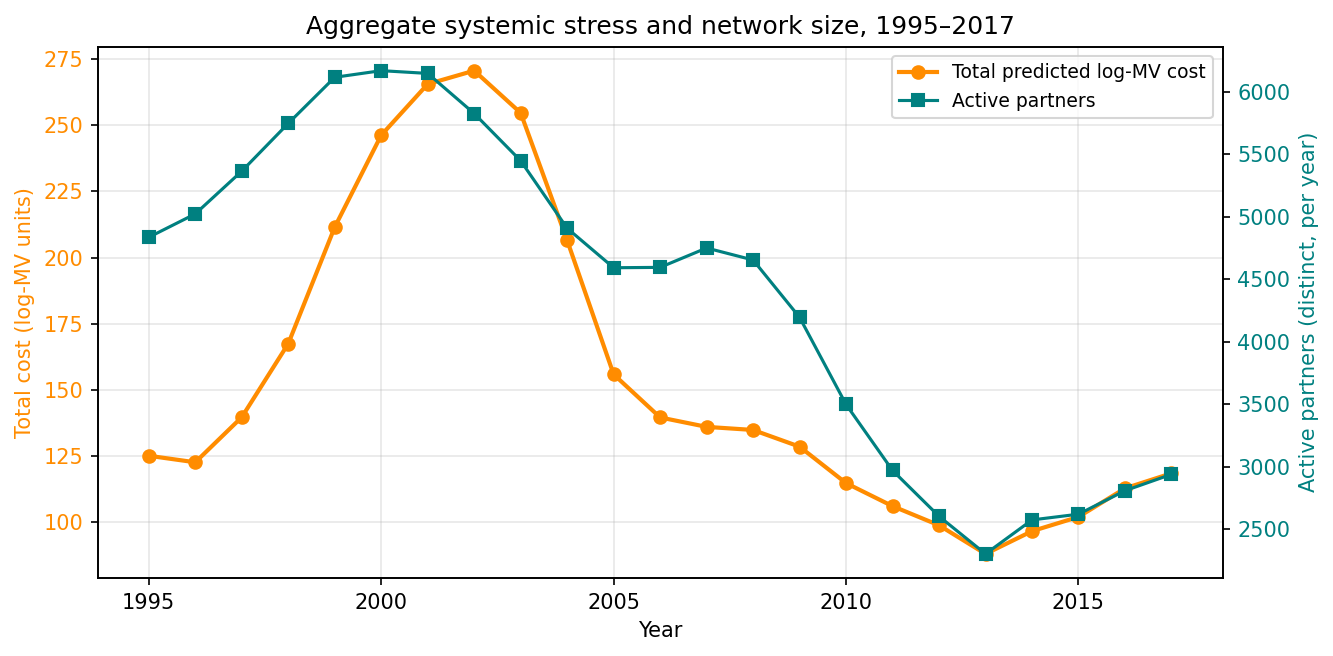
\includegraphics[width=0.80\textwidth]{fig_d5_system_stress.png}
\caption{Aggregate systemic stress (orange, left axis) and active-partner
count (teal, right axis), 1995--2017.  Both move with the alliance
activity cycle; the post-2008 contraction is pronounced on both
series.}
\label{fig:d5}
\end{figure}

\paragraph{Leaderboard persistence.}
Year-over-year retention of the top-20 systemic-critical set averages
71.4\%.  It is lowest in 2006 (50\%) and highest in 2001 (85\%).  Four
firms sit in the top-20 for at least 15 of 23 years: General Electric
(23/23), Microsoft (20), IBM (17), and Motorola Solutions (15).
Figure~\ref{fig:d1} renders the full rank trajectory for the 15 firms
with nine or more top-20 years.

\begin{figure}[H]
\centering
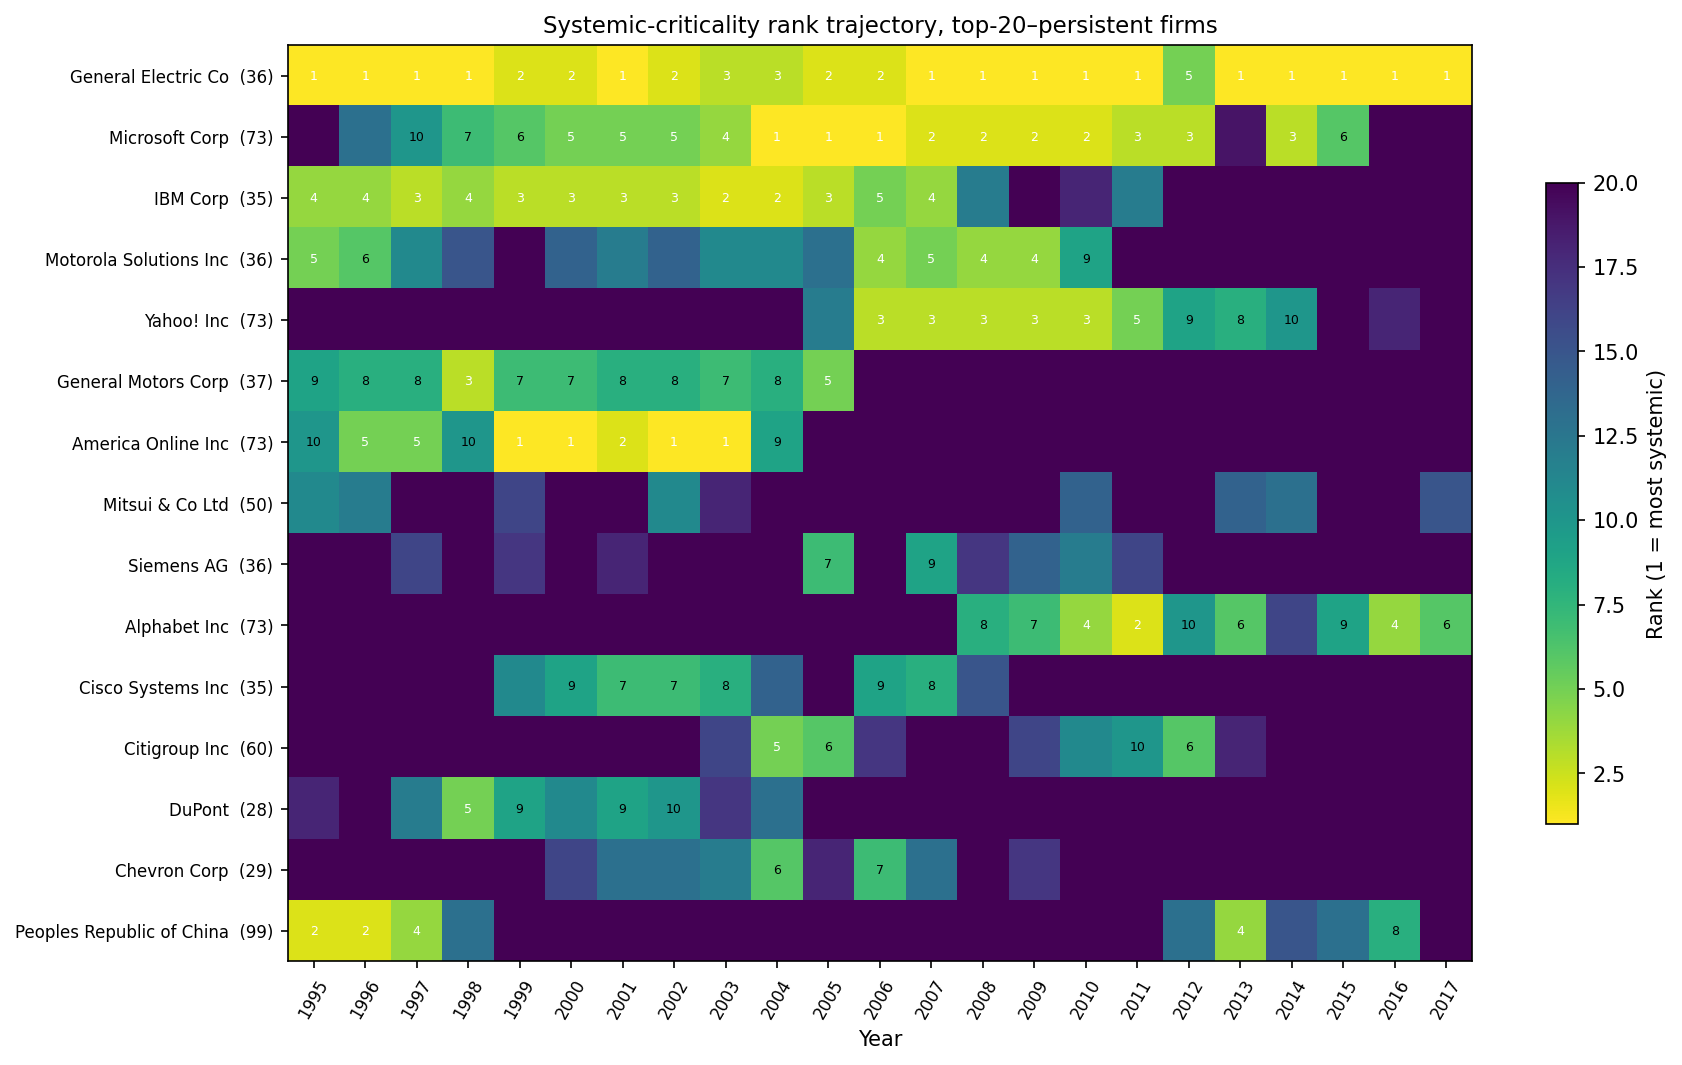
\includegraphics[width=0.96\textwidth]{fig_d1_rank_heatmap.png}
\caption{Systemic-criticality rank trajectory, 1995--2017, for the 15
firms with at least nine years in the top-20.  Colors encode rank
(1~=~most systemic); absent cells indicate years in which the firm
fell out of the rankable pool.}
\label{fig:d1}
\end{figure}

\paragraph{Risers and fallers.}
Restricting to partners that reached the top-100 in at least one year
removes fringe-to-fringe noise.  The largest rank gainers are
Oakley, Swisscom, Pegasystems, Tyson Foods, Biocon, Toppan Printing,
and Pall; Alphabet and Amazon enter the persistent top-20 from
earlier mid-tier positions.  Most of the largest rank
\emph{declines} (Exxon Corp, Daimler-Benz, Royal Dutch Petroleum,
Shell Transport~\&~Trading, NYNEX, ICI, Coopers~\&~Lybrand) are
pre-merger legacy tickers rather than genuine exits; reading against
their merged successors, these firms remain present in the
network.\footnote{Ticker persistence across ownership changes is an
  open integration problem for SDC Platinum identifiers.  Here we
  treat these entities honestly as observed---if CUSIPs vanish after a
  merger, they vanish from the panel---rather than backfill a
  hand-merged crosswalk.}

\paragraph{Industry concentration evolution.}
Figure~\ref{fig:d2} plots the SIC-2 Herfindahl index and the top-3 /
top-10 share of total predicted cost.  The HHI rises from 0.038 in
1996 to a dot-com-era peak of 0.067 in 2004, then relaxes to 0.049 in
2017.  Leadership shifts from SIC~36 (electronics) in the mid-1990s
to SIC~73 (business services and software) from 1998 onwards,
consistent with platform consolidation as the driver of systemic
concentration in the corrected panel.

\begin{figure}[H]
\centering
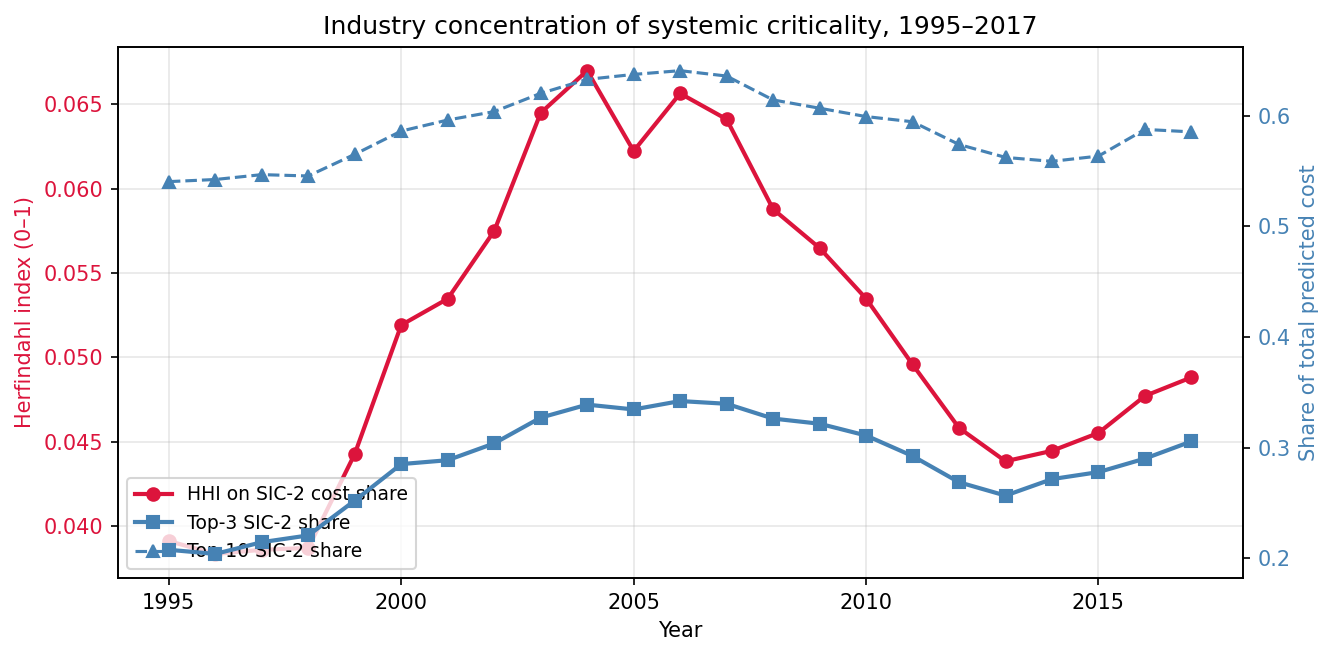
\includegraphics[width=0.86\textwidth]{fig_d2_concentration_over_time.png}
\caption{Industry concentration of systemic criticality.
Left axis: Herfindahl--Hirschman index on SIC-2 shares of total
predicted cost (red).  Right axis: top-3 and top-10 SIC-2 share
(blue).  Concentration peaks in 2004 and has declined modestly
since.}
\label{fig:d2}
\end{figure}

\paragraph{Compustat-matched share.}
Compustat-matched firms account for 32.7\% of total predicted cost in
1995 and 30.0\% in 2017, with a dot-com-era maximum of 39.1\% (2001)
and a post-2008 minimum of 28.6\% (2015).  The remainder is dominated
by sovereign entities (PRC, Singapore, UAE, Saudi Arabia),
private-equity vehicles (Blackstone, Carlyle), and non-US public
firms lacking a Compustat North-America match.  The meta-network is
decidedly not US-centric, and the Compustat share is roughly
stationary once the dot-com buildout is netted out.

% =====================================================================
\section{Robustness and Experiments}
\label{sec:robustness}

\subsection{\texorpdfstring{Top-$k$ sensitivity}{Top-k sensitivity}}

The top-5 cutoff is no longer an untested modeling choice.  Table
\ref{tab:topk} rebuilds the ranking at alternative cutoffs.  The
top-20 is identical for $k=3$ and $k=5$, and remains mostly stable for
larger cutoffs, though $k=1$ drops seven of the top-20 firms.

\begin{table}[H]
\centering
\footnotesize
\caption{Top-$k$ sensitivity of the 2017 systemic ranking.}
\label{tab:topk}
\begin{tabular}{lrrrr}
\toprule
$k$ & Edges & Partners & Spearman vs $k=5$ & Top-20 overlap \\
\midrule
1   & 1{,}754 & 1{,}504 & 0.940 & 13 \\
3   & 3{,}121 & 2{,}537 & 0.983 & 20 \\
5   & 3{,}690 & 2{,}939 & 1.000 & 20 \\
10  & 4{,}286 & 3{,}346 & 0.989 & 16 \\
20  & 4{,}642 & 3{,}559 & 0.985 & 16 \\
all & 4{,}918 & 3{,}721 & 0.984 & 16 \\
\bottomrule
\end{tabular}
\end{table}

\subsection{Null-model concentration}

We shuffle critical partners within dominant-layer bins and recompute
concentration over 100 simulations.  The observed top-20 cost share is
0.0648, above the null mean of 0.0512 and the null 95th percentile of
0.0536.  The observed HHI is 0.000826 versus a null mean of 0.000696.
Thus the concentration in the systemic ranking is not just an artifact
of the marginal edge-cost distribution.

\subsection{Estimator and ablation robustness}

Table~\ref{tab:robust} compares the primary ranking to estimator and
feature ablations.  The most important result is that legacy TWFE,
DMD-only, blended, and stacked-cohort estimates do not produce the same
ranking.  Legacy TWFE has $\rho=0.497$ with the primary ranking and
top-20 overlap 10/20; DMD-only has $\rho=0.596$ and overlap 8/20.
This is why the paper reports estimator disagreement rather than
presenting a single causal ranking.

\begin{table}[H]
\centering
\footnotesize
\caption{Estimator and ablation robustness, 2017 ranking.}
\label{tab:robust}
\begin{tabular}{lrrr}
\toprule
Variant & Spearman vs primary & Top-20 overlap & Top-20 churn \\
\midrule
Primary stacked/estimated       & 1.000 & 20 &  0 \\
Legacy TWFE weight              & 0.497 & 10 & 10 \\
Blended stacked/TWFE            & 0.869 & 12 &  8 \\
DMD-only, legacy available      & 0.596 &  8 & 12 \\
Layer-only, no partner features & 0.827 & 14 &  6 \\
No redundancy discount          & 0.945 & 15 &  5 \\
No counterfactual exposure      & 0.979 & 16 &  4 \\
Raw-degree proxy                & 0.777 & 13 &  7 \\
\bottomrule
\end{tabular}
\end{table}

\subsection{Backtest on observed partner exits}

The observed-exit backtest is deliberately conservative.  Among
partner exits in 1995--2016, top-5 predicted critical edges do not show
larger realized next-year market-value drawdowns; mean next-year
log-market-value change is positive in all rank buckets (top-5:
$+0.053$, rank 6--20: $+0.037$, rank $>$20: $+0.039$).  This means
the systemic score should be read as a structural exposure and stress
test, not as a validated one-year realized-drawdown predictor.

\subsection{System stress test}

In the 2017 stress test, removing the top five systemic partners
produces an aggregate model-implied market-value exposure of 192{,}800
in Compustat units, 31.8 times the random-removal mean.  Removing the
top ten produces 291{,}987, 24.2 times the random-removal mean.  The
systemic ranking also exceeds high-market-value, high-degree, and
high-eigenvector removal baselines, indicating that the meta-network
captures a dependency dimension not reducible to standard centrality or
firm scale.

% =====================================================================
\section{Implications}
\label{sec:implications}

\subsection{For corporate strategy: redundancy audits}

For any focal firm, the combination of its per-firm vulnerability table
and the aggregate meta-network identifies \emph{shared critical
partners}: partners whose loss would not only affect the focal firm but
would simultaneously affect many peers.  The practical action is a
redundancy audit.  A focal firm should identify partners that are both
locally hard to substitute and globally systemically critical, then
evaluate backup partners, long-term contracting, equity stakes, or
selective acquisition.

\subsection{For regulatory policy: concentration beyond market share}

Traditional antitrust and competition analysis measures concentration
through product-market shares.  The meta-network measures concentration
in alliance-channel dependency.  This is not a replacement for HHI or
market-definition analysis; it is an additional early-warning view of
where the alliance economy routes operational and commercialization
exposure through a small number of entities.

\subsection{For supply-chain resilience monitoring}

Supply-chain risk assessment usually follows direct supplier tiers.
The meta-network reveals a different risk: cross-portfolio dependence
on partners that may not be direct suppliers in the narrow procurement
sense but are structurally indispensable to multiple firms' alliance
portfolios.  The stress-test experiment shows that removing top
systemic partners is far more damaging in predicted aggregate exposure
than removing random partners or even simply large partners.

% =====================================================================
\section{Boundary Condition: From Dependency Map to Candidate Annotation}
\label{sec:downstream}

The systemic-criticality panel is a population-level map of
dependency hubs.  A natural downstream question is whether the same
partner-level quantities can personalize alliance recommendations
for individual focal firms.  We use the operational alignment
pipeline as a stress test of that interpretation.  The answer is
largely negative.  Candidate-side systemicity, tenure, and degree
features are useful annotations on a brokerage frontier, but they
do not produce a validated focal-specific ranking; in saturated
brokerage frontiers some of them even point away from realized new
$L_2$ partners.  This section therefore documents a boundary
condition of the systemic panel: it is an exposure map, not a
standalone recommender.

Operationally, two artifacts from this paper enter the alignment
pipeline that runs per-firm reports for the 7{,}626 Compustat-matched
focal firms.  The layer-specific exit weights of
Section~\ref{sec:method} weight the value side of a candidate-value
annotation, and the partner-level normalized in-degree from
Section~\ref{sec:findings} enters as a dependency-risk discount on
the candidate side.  We tested the multiplicative combination of
these annotations as an operational ranker and found that it does
not validate as one.  The retained object is a brokerage frontier
with descriptive durability and dependency annotations; the
systemic panel's role is annotation, not selection.

\subsection{A persistence-aware durable-rent score, as a tested
            operational hypothesis}

We first tested a persistence-aware durable-rent score motivated by
the companion DMD finding.  The score was designed to combine focal
brokerage opportunity with candidate tie-maintenance and
systemic-risk annotations:
\begin{align}
\text{durable\_value}(c)
   &= \text{brokerage}_{L_2}(f, c) \cdot w_{\text{tenure}}(c), \\
w_{\text{redundancy}}(c)
   &= \exp\!\bigl(-\rho \cdot \text{DepRisk}(c)\bigr),
\quad \rho = 1.5, \\
\text{score}(c)
   &= \text{durable\_value}(c) \cdot w_{\text{redundancy}}(c), \\
g(\text{R\&D}_{f})
   &= 1 + \alpha \cdot \mathbf{1}\{f \in Q^{\text{R\&D}}_{0.75}\},
\quad \alpha = 0.5.
\end{align}
Here $w_{\text{tenure}}(c) \in (0, 1)$ is an empirical-Bayes-shrunk
sigmoid of the candidate's $\log(1+\text{median tenure})$ z-scored
against its SIC--$L_2$ cohort baseline.  The shrinkage form is
$w = 0.5 + n / (n+\kappa) \cdot (\sigma(z) - 0.5)$ with $\kappa = 5$;
this prevents single-tie outliers from dominating via tiny SIC-cell
variance.  $\text{DepRisk}(c)$ is the candidate's normalized in-degree
in the 2017 systemic-criticality cross-section, with a ``not in
panel'' flag distinguishing structurally-zero risk from unobserved
risk.  $g(\text{R\&D}_f)$ is a per-focal absorptive-capacity
multiplier motivated by the L$_2$ sales premium's R\&D
stratification (companion paper, Section~4 / Figure~3B).

The score operationalizes the companion Hankel-DMD analysis's
persistence-vs-acquisition asymmetry: the L$_2$ sales premium is
associated with sustained ties, not freshly acquired ones, so a
candidate's demonstrated tie-maintenance behavior is treated as a
screening device on top of the structural opportunity.  The
diagnostic results below show that this multiplicative construction
should not be used as a ranker.

\paragraph{A note on the historical use of \texttt{DepRisk}.}
For the cross-sectional 2017 reporting, $\text{DepRisk}(c)$ is the
candidate's normalized in-degree in the 2017 systemic-criticality
cross-section.  For the historical out-of-time backtests in
Section~\ref{sec:phase9b-lite} (score years 2008--2013), the current
recommender implementation reads from the same 2017 cross-section
rather than from the year-specific annual systemic-criticality
panel.  The historical $\text{DepRisk}$ used in the backtest is
therefore a static 2017 overlay, not a temporally-aligned signal.
This is acknowledged here rather than hidden; an annual re-keying of
$\text{DepRisk}$ to the score-year row of \texttt{systemic\_criticality\_annual.csv}
is a cheap follow-up that does not change the qualitative findings
because $\text{DepRisk}$ enters only as an annotation and the
within-block direction is already reported in
Table~\ref{tab:within-block} as anti-correlated with realized choice
either way.

\subsection{Population-scale personalization diagnostic}

We ran the recommender on all 7{,}626 focal firms against their full
$L_2$ candidate pools at year 2017 (18{,}064{,}303 distinct
$(f, c)$ rows) and compared seven rankers and six blends on the
top-1 effective-distinct-candidates count
$N_{\mathrm{eff}} = 1 / \sum_c q_c^2$ (where $q_c$ is the share of
focal firms whose top-1 is candidate $c$):

\begin{table}[H]
\centering
\footnotesize
\caption{Personalization diagnostic across 7{,}626 focal firms.
$N_{\mathrm{eff}}^{\text{top-1}}$ is the effective number of
distinct top-1 candidates produced by each ranker.}
\label{tab:personalization}
\begin{tabular}{lrll}
\toprule
Ranker & $N_{\mathrm{eff}}^{\text{top-1}}$ & Top candidate & Top share \\
\midrule
\texttt{brokerage\_only}        & \textbf{1{,}811.9} & (no single dominant) & 0.13\% \\
\texttt{global\_degree\_l2}     & 1.001 & (single firm) & 99.95\% \\
\texttt{n\_current\_ties}       & 1.001 & (single firm) & 99.96\% \\
\texttt{w\_tenure\_only}        & 1.001 & MIT           & 99.96\% \\
\texttt{brokerage\_x\_tenure}   & 1.001 & (single firm) & 99.96\% \\
\texttt{raw\_score} (full)      & \textbf{1.000} & Stanford University & \textbf{100.0\%} \\
Blends $\alpha \in [0.25, 1.0]$ & 1.000 & Stanford & 100.0\% \\
Residual rank ($\alpha = 0$)    & 1.001 & (single firm) & 99.96\% \\
\bottomrule
\end{tabular}
\end{table}

The full multiplicative durable-rent score collapses to a single
candidate (Stanford University) for every one of the 7{,}626 focal
firms.  This is not an artifact of any one feature: removing
$w_{\text{tenure}}$ produces collapse onto a different single
candidate (MIT, under the brokerage-saturated tail).  The collapse
persists when stratified by candidate type (each candidate-type
stratum has its own dominant pick).  Residualizing the raw score
against candidate-global features cannot recover personalization,
because when the score is already dominated by candidate-side
features, the within-focal rank of any candidate-side residual is
identical across focals.

The single feature that produces a focal-specific top-1 ranking is
$\text{brokerage}_{L_2}(f, c)$ itself, which depends on $f$ by
construction; it yields $N_{\mathrm{eff}} \approx 1{,}812$, with the
most-frequent top-1 candidate appearing in only $\approx 10$ of the
7{,}626 focal firms' lists.

This should not be interpreted as proof of rank validity.  Because
brokerage is often saturated at its maximum value, top-choice
diversity can arise from deterministic ordering inside very large
tie blocks rather than from any meaningful focal-specific score
gradient.  Section~\ref{sec:phase9b-lite} therefore audits the
saturated frontier directly: for every realized in-pool dyad we
compute $r_{\min}$ and $r_{\max}$, the minimum and maximum
within-pool brokerage rank of the realized partner, and report the
expected hit rate under random tie-breaking.  The brokerage score
is best understood as a focal-specific gating variable that
defines the frontier, not as a fully-resolved ranker over it.

\subsection{Methodological reading}

The collapse has a specific and useful interpretation.  The systemic
panel's normalized in-degree, the candidate's tie-maintenance
record, and global degree statistics are all candidate-side
features: they do not vary across focals.  In a candidate pool where
the focal-specific signal ($\text{brokerage}_{L_2}$) saturates at 1.0
for almost all candidates --- which it does for the vast majority of
sparse-portfolio focals --- multiplicative combinations of any
candidate-side features produce identical within-focal rankings, and
therefore identical top-1 picks.  The systemic panel is informative
about \emph{which firms are dependency hubs}; it is not, on its own,
informative about \emph{which firm is the right partner for a
specific focal}.

The downstream pipeline therefore separates two questions.
$\text{brokerage}_{L_2}$ defines a focal-specific brokerage frontier
(the set of candidates with non-overlapping $L_2$ neighborhoods).
Within the saturated frontier, the current in-data features do not
provide a validated total ordering; ranking by brokerage alone is a
frontier-membership statement, not a focal-specific selection score.
The \emph{value} attached to a candidate, conditional on frontier
membership, draws on the systemic panel and the relational-capability
features as descriptive scalars.  The systemic-criticality panel from
this paper retains its operational role --- as a dependency-exposure
overlay on the brokerage frontier, not as the rank itself.

\subsection{Cheap interaction features do not break the collapse}
\label{sec:interaction-features}

A natural objection is that the Week-2A diagnostic was conducted with
a feature set that was almost entirely candidate-side, and that adding
genuine focal-conditional interaction features should restore
personalization.  We tested this.  On the same 18M-row scoring frame
we computed seven $(f, c)$-conditional features that are cheap to
construct from the existing data --- partner-set overlap counts,
Jaccard similarity, share of focal partners that are candidate
partners, same-SIC2 indicator, same-SIC1 indicator, SIC2 nominal
distance, and nation match --- and re-ran the personalization
diagnostic with each feature alone, with each feature combined with
$\text{brokerage}_{L_2}$ via within-focal rank-sum, and with all
features combined.

\begin{table}[H]
\centering
\footnotesize
\caption{Personalization diagnostic with cheap focal-conditional
interaction features added.  None of the seven new features beats
$\text{brokerage}_{L_2}$ alone; combinations tie or underperform it.}
\label{tab:interaction}
\begin{tabular}{lrll}
\toprule
Ranker & $N_{\mathrm{eff}}^{\text{top-1}}$ & Top candidate & Top share \\
\midrule
\texttt{brokerage\_only} (Week-2A baseline) & \textbf{1{,}811.9} & Acuity Brands Inc & 0.13\% \\
\texttt{jaccard\_only}                & 1{,}734.1 & New York Power Authority & 0.20\% \\
\texttt{n\_shared\_partners\_only}    & 1{,}630.3 & General Electric Co      & 0.43\% \\
\texttt{share\_focal\_in\_c\_only}    & 1{,}630.3 & General Electric Co      & 0.43\% \\
\texttt{nation\_match\_only}          & 1{,}521.1 & Twitter Inc              & 0.16\% \\
\texttt{same\_sic2\_only}             & 1{,}125.5 & HSBC                     & 0.39\% \\
\texttt{broker\_x\_jaccard} (rank-sum)  & 1{,}732.2 & New York Power Authority & 0.20\% \\
\texttt{broker\_x\_shared} (rank-sum)   & 1{,}626.5 & General Electric Co      & 0.43\% \\
\texttt{broker\_x\_nation} (rank-sum)   & 1{,}521.6 & University of Guelph     & 0.16\% \\
\texttt{broker\_x\_sic2} (rank-sum)     & 1{,}125.5 & HSBC                     & 0.39\% \\
\texttt{full\_interaction} (4-feature rank-sum) & 831.2 & Everi Holdings Inc & 0.84\% \\
\texttt{raw\_score} (Week-2A full)    & 1.000 & Stanford University & 100.0\% \\
\bottomrule
\end{tabular}
\end{table}

The mechanism is simple but not obvious from the formulation.  Each
interaction feature is focal-conditional in its values, but the
\emph{argmax} of any feature also has to vary across focals.
Partner-set features rank degree hubs (GE) high almost everywhere
even though the values per focal differ; \texttt{same\_sic2} and
\texttt{nation\_match} are partitions whose ``match'' set has
random within-partition order, so whichever same-SIC firm appears
first wins every focal in that SIC (HSBC dominates among financial
focals).  Combining brokerage with these features via rank-sum
\emph{halves} the personalization in the worst case ($N_{\mathrm{eff}}
\approx 831$) because the interaction features dilute brokerage's
focal-specificity with their own globally-popular tops.

The implication is that $\text{brokerage}_{L_2}(f, c)$ is the
personalization ceiling under in-data features.  To exceed it would
require new data the current pipeline does not expose: a tie-formation
hazard model conditional on $(f, c)$ covariates, cross-portfolio
similarity (patent-class, earnings-call topic embeddings), geographic
or supply-chain proximity beyond nation, or board-interlock and M\&A
history.  These are real options for a follow-on phase but each
requires either external data or substantial modeling work.

\subsection{Out-of-time validation: the saturated frontier and
            anti-correlated annotations}
\label{sec:phase9b-lite}

We backtest the brokerage-frontier recommender on six years of
realized new $L_2$ ties ($T \in \{2009, \ldots, 2014\}$).  For each
year $T$, the recommender is run at score year $T-1$ (no $T$-year
data leakage).  Realized new $L_2$ dyads are partitioned into a
seven-class coverage taxonomy.  Pooled across the six backtest
years (1{,}638 directed realized rows = 819 unique dyads):

\begin{table}[H]
\centering
\footnotesize
\caption{Coverage breakdown for realized new $L_2$ dyads,
2009--2014. Only candidates with prior $L_2$ activity are reachable
by the brokerage-frontier recommender.}
\label{tab:coverage}
\begin{tabular}{lrr}
\toprule
Coverage class & N rows & \% of 1{,}638 \\
\midrule
\texttt{focal\_not\_compustat}                & 1{,}183 & 72.2\% \\
\texttt{candidate\_genuine\_new\_L2\_entrant} &   206 & 12.6\% \\
\textbf{\texttt{candidate\_in\_pool}} (reachable) &  120 &  \textbf{7.3\%} \\
\texttt{candidate\_prior\_L2\_excluded\_by\_pool} &  62 &  3.8\% \\
\texttt{candidate\_prior\_SDC\_no\_L2}        &    63 &  3.8\% \\
\texttt{candidate\_prior\_nonL2\_same\_focal} &     4 &  0.2\% \\
\texttt{candidate\_unmatched}                 &     0 &  0.0\% \\
\bottomrule
\end{tabular}
\end{table}

Two distinct limitations are visible in Table~\ref{tab:coverage}.
The first is a \emph{focal-side scope boundary}: 72.2\% of directed
realized rows fall outside the Compustat-focal evaluation universe,
which is intentional --- market-value outcomes require Compustat
coverage --- but caps the share of new $L_2$ activity any
Compustat-focal recommender can ever address.  The second is a
\emph{candidate-side reach bottleneck} conditional on focal
eligibility: of the rows with Compustat focals, only 120 have a
candidate in the prior-$L_2$ pool, while 206 are genuine new $L_2$
entrants, 63 have prior SDC activity but no prior $L_2$, and 62 have
prior $L_2$ but are excluded by the rolling-window pool rule.  Under
this operational definition, prior non-$L_2$ same-focal conversion
is not a major source of new $L_2$ formation (4 rows out of 1{,}638),
which does not support a ``recommend cross-layer conversions''
extension as a high-yield intervention here.

For the 119 in-pool dyads, brokerage saturates as expected: 99\% of
within-focal candidates have $\text{brokerage}_{L_2} = 1.0$, with
median tie-block size 2{,}896.  We compute the realized partner's
within-tie-block percentile under each annotation,
$P^a_{fc^\star t} = \bigl[\#\{c \in \mathcal B : a < a^\star\}
+ 0.5 \cdot \#\{c \in \mathcal B : a = a^\star\}\bigr] / |\mathcal B|$.
Random ordering inside the block implies $\mathbb E[P^a] = 0.5$.
Mean percentile per annotation, with 95\% CI from a focal-clustered
bootstrap (1{,}000 reps):

\begin{table}[H]
\centering
\footnotesize
\caption{Within-saturated-block annotation percentiles for the
realized partner ($N$ in-pool dyads, focal-clustered bootstrap CI).
CIs in bold exclude the 0.5 random baseline.  Higher $P^a$ means
the realized partner sits higher in the within-block distribution
of the named annotation.}
\label{tab:within-block}
\begin{tabular}{lrrcc}
\toprule
Annotation & $N$ & Mean $P^a$ & 95\% CI & Reading \\
\midrule
\texttt{n\_hist\_ties}                  & 119 & \textbf{0.820} & \textbf{[0.781, 0.857]} & realized partners are degree-heavy \\
\texttt{n\_current\_ties}               & 119 & \textbf{0.820} & \textbf{[0.772, 0.861]} & same \\
\texttt{candidate\_degree\_all}         & 119 & \textbf{0.819} & \textbf{[0.772, 0.861]} & same \\
\texttt{candidate\_degree\_l2}          & 119 & \textbf{0.745} & \textbf{[0.693, 0.793]} & moderate \\
\texttt{w\_tenure\_smooth}              & 119 & \textbf{0.221} & \textbf{[0.178, 0.274]} & lower tenure than block median \\
\texttt{w\_redundancy}                  & 119 & \textbf{0.216} & \textbf{[0.174, 0.257]} & lower redundancy than block median$^\dagger$ \\
\texttt{annotated\_value\_synthetic}    & 119 & \textbf{0.154} & \textbf{[0.119, 0.192]} & multiplicative product compounds the two \\
\texttt{dep\_risk}                      &  81 & \textbf{0.084} & \textbf{[0.072, 0.096]} & lower observed dependency risk$^\ddagger$ \\
\bottomrule
\end{tabular}
\end{table}

\vspace{-0.4em}
\noindent\footnotesize $^\dagger$ \texttt{w\_redundancy} percentile
includes all 119 dyads: candidates with unobserved $\text{DepRisk}$
default to $w_{\text{redundancy}} = 1.0$ (the maximum), so the
realized partner being in the bottom $\sim$22\% means it is more
often in the small minority of candidates with observed positive
$\text{DepRisk}$ (i.e., $w_{\text{redundancy}} < 1.0$).
$^\ddagger$ \texttt{dep\_risk} percentile is computed over the
$N=81$ subsample where the realized partner's $\text{DepRisk}$ is
observed (i.e., the partner appears in the 2017
systemic-criticality cross-section); among that subsample, the
realized partner is at the low end of the observed-risk
distribution.  The two readings are consistent: realized partners
overlap meaningfully with the observed-$\text{DepRisk}$ subset, and
within that subset they sit at the low-systemic end.\normalsize

Three readings are supported by Table~\ref{tab:within-block}.  First,
candidate degree (current, historical, and $L_2$-specific) is
positively associated with the realized partner inside the saturated
brokerage frontier, with mean percentile $\approx 0.82$ and tight
CIs that exclude the random baseline.  Second, the recommender's
durability annotations point in the opposite direction from the
durable-rent hypothesis: the realized partner is more often in the
bottom quintile of \texttt{w\_tenure\_smooth} and in the small
minority with observed positive $\text{DepRisk}$ (so
\texttt{w\_redundancy} below the block median); within the
observed-$\text{DepRisk}$ subset itself the realized partner sits
at the low-risk end.  The multiplicative
\texttt{annotated\_value\_synthetic} compounds these patterns to
mean $P = 0.154$.  Third, the Hankel-DMD analysis is consistent
with this: it says \emph{sustained} $L_2$ brokerage is associated
with later sales, especially for R\&D-intensive focals; it does
not imply that already-tenured candidates should be selected for
new $L_2$ ties, and our diagnostic suggests that, in this dataset,
firms tend to select fresh, low-history, less-systemic partners
when forming new $L_2$ alliances.  The recommender's value/risk
annotations are therefore best read as descriptive labels on the
brokerage frontier, not as priority signals for selection.

We also estimate sales-association at the focal-year level
(maximum within-block percentile per focal, OLS with year fixed
effects + Compustat controls $\log\text{sales}_t$,
$\log\text{assets}_t$, R\&D intensity, and the count of in-pool
realized partners).  All annotations have $\beta_h$ confidence
intervals that overlap zero at $h \in \{2, 4\}$ ($N$ = 35--43
focal-years per cell), so this small-$N$ test is uninformative for
sales association.  We report the betas in
\texttt{week2b\_sales\_regression.csv} but make no claim of sales
lift from any annotation.

% =====================================================================
\section{Limitations}
\label{sec:limitations}

\paragraph{Structural exposure, not observed cascade realization.}
The meta-network aggregates predicted exposure scores.  The observed
exit backtest does not validate larger one-year market-value drawdowns
for top-ranked edges.  The ranking is therefore best interpreted as a
stress-testing and dependency-mapping tool.

\paragraph{Estimator disagreement.}
Legacy TWFE and stacked-cohort estimates disagree materially.  TWFE
recovers a negative and statistically significant L$_2$ estimate, but
the stacked-cohort estimate is positive and insignificant.  The primary
ranking uses the conservative stacked reference, while robustness files
report the TWFE ranking separately.

\paragraph{First-order counterfactual centrality.}
The $\Delta c^{(\lambda)}$ fields approximate betweenness exposure by
allocating focal layer-betweenness across partners according to
layer-specific tie strength.  Exact recomputation of betweenness after
every possible partner deletion would be computationally much more
expensive and is left for targeted follow-up on the top-ranked edges.

\paragraph{Asymmetric coverage.}
Focal firms are Compustat-matched because market-value losses require
financial outcomes.  Critical partners can be any SDC participant.
This preserves the full-graph protocol but means private and foreign
partners can be ranked as systemically critical without receiving their
own complete financial vulnerability audit.

\paragraph{Top-5 truncation.}
Top-$k$ sensitivity shows stability from $k=3$ to $k=5$ but some churn
at $k=1$ and $k \geq 10$.  The top-5 cutoff is useful and stable enough
for the main ranking, but policy or firm-level applications should
inspect the full \texttt{critical\_edges\_panel.parquet} artifact.

\paragraph{Candidate-side, not focal-conditional, by construction.}
The panel's normalized in-degree, mean predicted cost, and layer mix
are properties of the partner alone, not of any specific
focal-partner pair.  They cannot personalize an operational alignment
recommender on their own (Section~\ref{sec:downstream},
Table~\ref{tab:personalization}): downstream consumers should rank
candidates by a focal-specific signal such as $\text{brokerage}_{L_2}(f, c)$
and use the systemic panel as a value scalar attached to the
brokerage-ranked top-$k$, not as the rank itself.  This is a feature
of the panel's level of analysis (the partner) rather than a defect:
the panel is a population map of dependency hubs, not a per-firm
recommender.

% =====================================================================
\section{Conclusion}

The corrected systemic-criticality analysis turns the prototype into a
reproducible annual dependency panel.  It fixes CUSIP identity leakage,
distinguishes total generated reports from non-empty active dependency
reports, replaces layer constants with partner-specific counterfactual
features, and reports estimator disagreement rather than hiding it.
End-to-end consistency is preserved: the aggregate
\texttt{critical\_edges\_panel.parquet} and all 7{,}626 per-firm
\texttt{stress.md} reports were regenerated from the same scorer, so
the systemic-criticality view at the population level and the
vulnerability view at the firm level can be cross-read without
silent discrepancies.

The resulting meta-network identifies firms and entities whose alliance
positions make them common dependencies across many portfolios.  It is
most useful as a structural stress test: a way to ask which partner
failures would concentrate exposure across firms, industries, and
countries.  The annual panel reported in
Section~\ref{sec:annual} adds a temporal dimension to that question:
the leaderboard is moderately stable (71\% year-over-year top-20
retention) but not static, and concentration peaked during the
dot-com era before relaxing.

The downstream recommender audit (Section~\ref{sec:downstream})
clarifies the level of analysis.  Systemic criticality is
informative about common dependency hubs, but partner-level
systemicity does not personalize focal-firm alliance choice.  In
saturated brokerage frontiers, candidate-side annotations can even
point away from realized new $L_2$ partners.  The appropriate use
of the panel is therefore as a structural stress-test and
dependency-annotation layer, not as a standalone alliance recommender.

The next empirical step is targeted validation on the top systemic
partners using exact deletion recomputation and richer event-study
designs around observed exits, together with a follow-on pipeline
that addresses entry --- not just choice among incumbents --- since
roughly three quarters of realized new $L_2$ ties involve focals or
candidates outside the current Compustat-and-prior-$L_2$ scope.

We frame the contribution as three claims:
\begin{enumerate}
  \item \textbf{Measurement contribution.} An identity-clean annual
  systemic-criticality meta-network for the multiplex alliance
  economy, with partner-specific exposure scoring.
  \item \textbf{Structural finding.} Systemic dependency is
  concentrated in interpretable partners, industries, and time
  periods, and is not reducible to firm size or standard centrality.
  \item \textbf{Boundary condition.} The same systemic panel should
  not be mistaken for a focal-firm recommender; downstream tests
  show candidate-side systemicity and durability annotations do not
  validate as selection ranks.
\end{enumerate}

\bibliographystyle{apalike}
\begin{thebibliography}{20}

\bibitem[Ahuja(2000)]{ahuja2000}
Ahuja, G. (2000).
\newblock Collaboration networks, structural holes, and innovation: A
longitudinal study.
\newblock \emph{Administrative Science Quarterly}, 45(3):425--455.

\bibitem[Anand and Khanna(2000)]{anand2000}
Anand, B.~N. and Khanna, T. (2000).
\newblock Do firms learn to create value? The case of alliances.
\newblock \emph{Strategic Management Journal}, 21(3):295--315.

\bibitem[Burt(1992)]{burt1992}
Burt, R.~S. (1992).
\newblock \emph{Structural Holes: The Social Structure of Competition}.
Harvard University Press.

\bibitem[Callaway and Sant'Anna(2021)]{callawaysantanna2021}
Callaway, B. and Sant'Anna, P.~H.~C. (2021).
\newblock Difference-in-differences with multiple time periods.
\newblock \emph{Journal of Econometrics}, 225(2):200--230.

\bibitem[Coleman(1988)]{coleman1988}
Coleman, J.~S. (1988).
\newblock Social capital in the creation of human capital.
\newblock \emph{American Journal of Sociology}, 94:S95--S120.

\bibitem[de Chaisemartin and D'Haultf{\oe}uille(2020)]{dechaisemartin2020}
de Chaisemartin, C. and D'Haultf{\oe}uille, X. (2020).
\newblock Two-way fixed effects estimators with heterogeneous
treatment effects.
\newblock \emph{American Economic Review}, 110(9):2964--2996.

\bibitem[Dyer and Singh(1998)]{dyersingh1998}
Dyer, J.~H. and Singh, H. (1998).
\newblock The relational view: Cooperative strategy and sources of
interorganizational competitive advantage.
\newblock \emph{Academy of Management Review}, 23(4):660--679.

\bibitem[Goodman-Bacon(2021)]{goodmanbacon2021}
Goodman-Bacon, A. (2021).
\newblock Difference-in-differences with variation in treatment
timing.
\newblock \emph{Journal of Econometrics}, 225(2):254--277.

\bibitem[Gulati(1995)]{gulati1995}
Gulati, R. (1995).
\newblock Social structure and alliance formation patterns: A
longitudinal analysis.
\newblock \emph{Administrative Science Quarterly}, 40(4):619--652.

\bibitem[Kale et~al.(2002)]{kale2002}
Kale, P., Dyer, J.~H., and Singh, H. (2002).
\newblock Alliance capability, stock market response, and long-term
alliance success: The role of the alliance function.
\newblock \emph{Strategic Management Journal}, 23(8):747--767.

\bibitem[Lavie(2007)]{lavie2007}
Lavie, D. (2007).
\newblock Alliance portfolios and firm performance: A study of value
creation and appropriation in the U.S. software industry.
\newblock \emph{Strategic Management Journal}, 28(12):1187--1212.

\bibitem[Phelps(2010)]{phelps2010}
Phelps, C.~C. (2010).
\newblock A longitudinal study of the influence of alliance network
structure and composition on firm exploratory innovation.
\newblock \emph{Academy of Management Journal}, 53(4):890--913.

\bibitem[Sun and Abraham(2021)]{sunabraham2021}
Sun, L. and Abraham, S. (2021).
\newblock Estimating dynamic treatment effects in event studies with
heterogeneous treatment effects.
\newblock \emph{Journal of Econometrics}, 225(2):175--199.

\bibitem[Uzzi(1997)]{uzzi1997}
Uzzi, B. (1997).
\newblock Social structure and competition in interfirm networks: The
paradox of embeddedness.
\newblock \emph{Administrative Science Quarterly}, 42(1):35--67.

\end{thebibliography}

\end{document}
